\documentclass{article}
\usepackage{graphicx}
\graphicspath{ {Plots/} }
\usepackage[export]{adjustbox}
\usepackage[leftcaption]{sidecap}
\usepackage{amssymb}
\usepackage[utf8]{inputenc}

\title{Statistical Methods in Infectious Disease Modeling}
\date{2017-04-20}
\author{Kaitlyn Stocker}

\begin{document}

\maketitle
\pagenumbering{gobble}
\newpage
\pagenumbering{arabic}
\tableofcontents
\newpage
%notes: 
%-write a 3 sentence (short) intro for each section
%- add references asap
%- convert all simulated examples to the same example - use measles the whole way

\section{Introduction}
%should include general info about infectious disease, general info about statistical inference (overview of MLE and Bayes

\section{Modeling and Inference for Infectious Disease}
\subsection{Deterministic Models}
%talk about die-outs, endemic equilibrium, etc. 
\subsection{Stochastic Models}
\subsubsection{Chain Binomial}
\subsubsection{TSIR}
\subsubsection{Susceptible Reconstruction}
In previous exercises, I had access to perfect and complete simulated data. While having such complete data is convenient, it is not realistic. Data gathered in real-world situations is much less inference-ready than the simulated data I have been using thus far.

Real data deviates from simulated data in a number of significant ways. For one thing, real data is incomplete. Not all cases of a disease are reported, so the number of infecteds at any given time point must be estimated using the number of reported cases multiplied by the reporting rate. There is typically no information about the true number of susceptible or recovered individuals, as collecting this information would be extremely impractical and cost-prohibitive. 

In order to run any kind of meaningful inference on epidemic data, it is necessary to have at minimum the infected and susceptible dynamics over time. Using the reported cases and the rate at which cases are reported, it is easy enough to construct the infected class dynamics. However, reconstructing the susceptible class dynamics is not so straight-forward. 

In order to reconstruct the susceptible class dynamics, let's first define the model. I will continue with the basic SIR model, but this time I am going to add in birth dynamics. The addition of birth dynamics into the susceptible class are crucial to the susceptible reconstruction process. To do this, I will define $B_{t-d}$ as the number of births at time $t-d$. Since infants are born with natural immunity from their mothers, there is a time delay (denoted by $d$) between when a baby is born and when it enters the susceptible class. The length of this delay is dependent on the disease. As before, I define the size of the infected class at a given time point $t$ to be $I_{t}, \in{\{1,...,T\}}$. Similarly, I define the size of the susceptible class at a given time point $t$ to be $S_{t} \in{\{1,...,T\}}$. Equations 12 and 13 give the model specifications. 

\begin{equation}
I_{t} = \beta S_{t-1} I_{t-1}
\end{equation}
\begin{equation}
S_{t} = B_{t-d} + S_{t-1} - I_{t}
\end{equation}

In equation 14 I allow $I_{t}$ to be a product of the number of reported cases, $C_{t}$ and $\rho_{t}$, the reporting rate at time $t$. I define $\rho$ such that when $\rho_{t} =1$, the number of true cases has been fully reported. When $\rho_{t} > 1$, the number of true cases has been underreported. Additionally, I assume that $\rho_{t}$ follows a probability distribution with  $E(\rho_{t}) = \rho$.

\begin{equation}
I_{t} = \rho_{t}C_{t}
\end{equation}

Substituting equation 14 into equation 13, we get: 

\begin{equation}
S_{t} = B_{t-d} + S_{t-1} -  \rho_{t} C_{t}
\end{equation}

If we define $E(S_{t})=\bar{S}$, then we can define a new variable $Z_{t}$ such that $S_{t} = \bar{S} + Z_{t}$, with $E(Z_{t})=0$. In this way, $Z_{t}$ is the deviations from the mean of $S_{t}$. $Z_{t}$ therefore follows the same recursive relationship as $S_{t}$, and can be defined as follows:

\begin{equation}
Z_{t} = B_{t-d} + Z_{t-1} -  \rho_{t} C_{t}
\end{equation}

If we allow $Z_{0}$ to be the initial value of Z, we can rewrite the previous equation to look like the following:

\begin{equation}
Z_{t} = Z_{0} + \sum_{i=1}^{t} B_{i-d} - \sum_{i=1}^{t} \rho_{i}C_{i}
\end{equation}

To de-clutter this notation, allow $Y_{t}=\sum_{i=1}^{t} B_{i-d}$ and $X_{t}= \sum_{i=1}^{t}C_{i}$. Additionally, we will assume a constant reporting rate. Now we can rewrite equation 17 as a simple linear regression equation:

\begin{equation}
Y_{t} = -Z_{0} + Z_{t} + \rho X_{t}
\end{equation}

Thus we have a linear regression equation relating cumulative births ($Y_{t}$) to cumulative reported cases ($X_{t}$). The susceptible dynamics $Z_{t}$ are the regression remainder to equation 18, and can thus be fully reconstructed. 

\paragraph{Simulated Susceptible Reconstruction Example}
In order to validate the accuracy of the susceptible reconstruction method taken from \{citation\}, I first used the method on simulated data. This way, I was able to compare the reconstructed susceptible dynamics to the true, simulated dynamics. 

I first simulated an infection with transmission rate $\beta = 1.66$ and recovery rate $\gamma = 1/2.2$ using the previously defined TSIR model, with one modification. I added birth dynamics to allow the use of susceptible reconstruction. I simulated births using a birth rate of 12 births per 1,000 people annually \{citation\}. 

Following the given method for reconstructing susceptible dynamics, I took the regression remainder from equation 18 and obtained $Z_{t}$. Figure \ref{fig:ZvsS} shows the reconstructed dynamics plotted alongside the true susceptible dynamics. The curves are equivalent, but as per definition $Z_{t}$ is centered around zero. 

\begin{figure}[htbp]
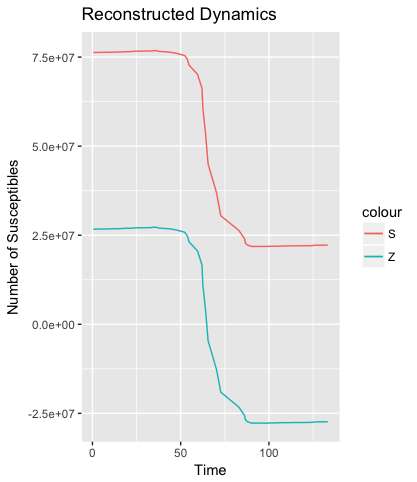
\includegraphics[scale=.5, center]{ZvsSplot.png}
\caption{Comparison of reconstructed susceptible dynamics, $Z$, and the true susceptible dynamics $S$ from the original simulation.}
\label{fig:ZvsS}
\end{figure}

In order to fully reconstruct the susceptible dynamics, it would be necessary to know $\bar{S}$. However, it is not possible to compute the mean number of susceptibles directly, as we are assuming we do not have any data about the true susceptible dynamics. Therefore, I had to instead infer $\bar{S}$ along with the other model parameters ($\beta$ and $\gamma$) when I performed Bayesian Inference. 

I defined the prior on $\bar{S}$ to be normal with a mean of one fifth the initial population size and a standard deviation that was half of the mean. In other words, if we allow $N_{0}$ to be the initial population size, then I defined the prior on $\bar{S}$ as follows: $\bar{S} \sim Normal(\frac{N_{0}}{5}, \frac{N_{0}}{10})$. I then proceeded to replace any instance of $S_{t}$ in the model definition with the equivalent expression $\bar{S} + Z_{t}$. 

After running inference on my reconstructed susceptible dynamics, I took the upper and lower bounds from the $95\%$ Credible Interval of $\bar{S}$ and used those values to obtain upper and lower bounds on the true susceptible dynamics. \ref{fig:SR} shows a plot of the true susceptible dynamics (from the simulation) contained within the upper and lower bounds of the $95\%$ credible interval for the reconstructed dynamics. The true values of $\beta$ and $\gamma$ were also contained within their respective $95\%$ credible intervals. 

\begin{figure}[htbp]
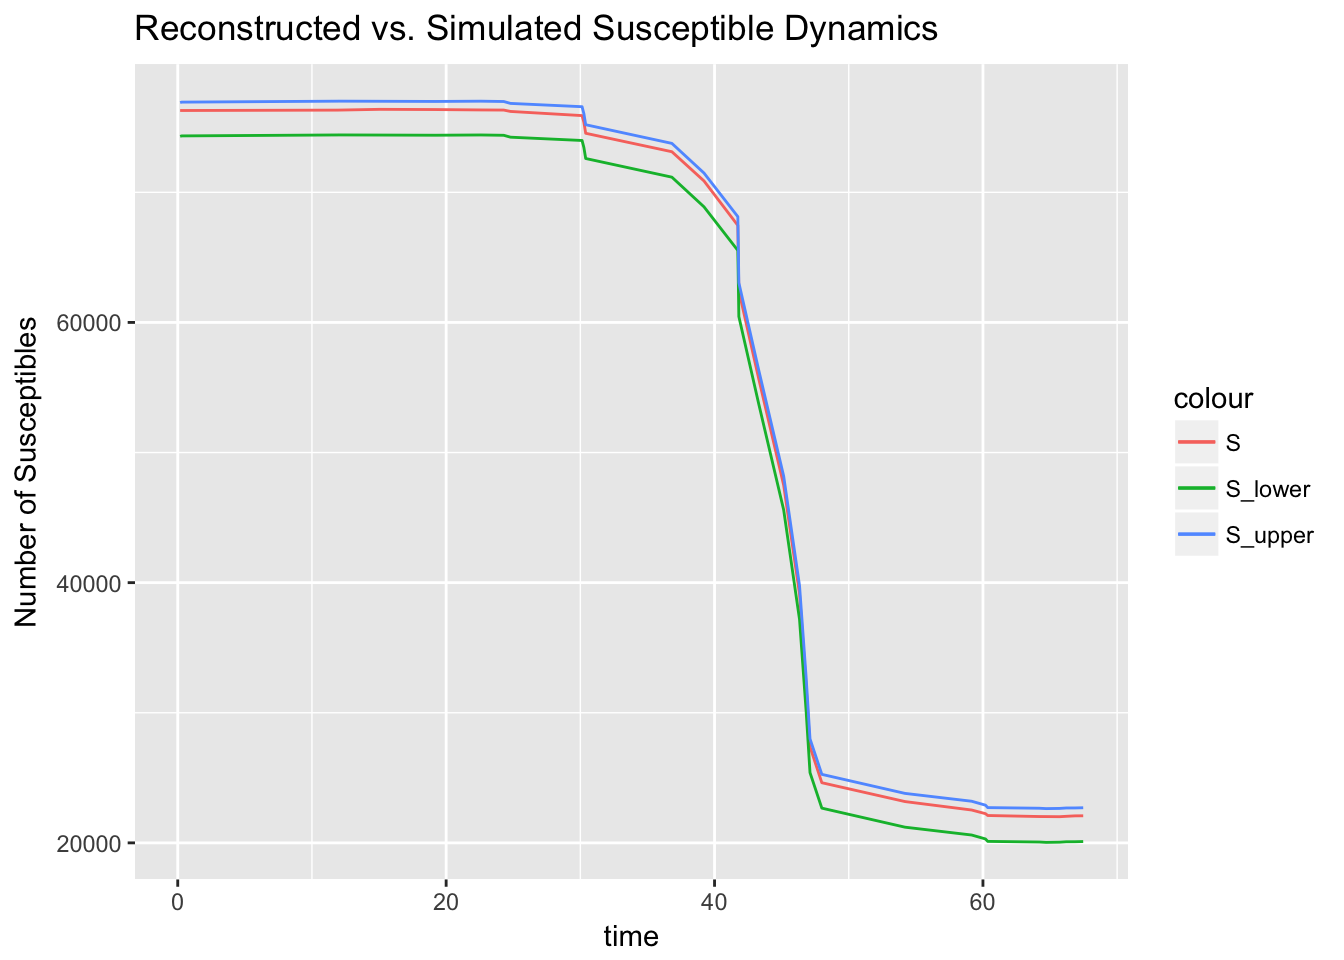
\includegraphics[scale=.25, center]{SRplot.png}
\caption{Plot of the true, simulated susceptible dynamics with the upper and lower estimated susceptible dynamics. The upper and lower bounds were obtained by taking the upper and lower limits of the 95\% credible interval for the mean number of susceptibles, and adding each value to $Z_{t}$. The true number of susceptibles (in red) is clearly contained within the upper and lower bounds of the reconstructed susceptible dynamics.}
\label{fig:SR}
\end{figure}


\subsection{Spatial Models}

\section{Application to Measles}

\section{Results}

\end{document}